\begin{figure}
  \centering
  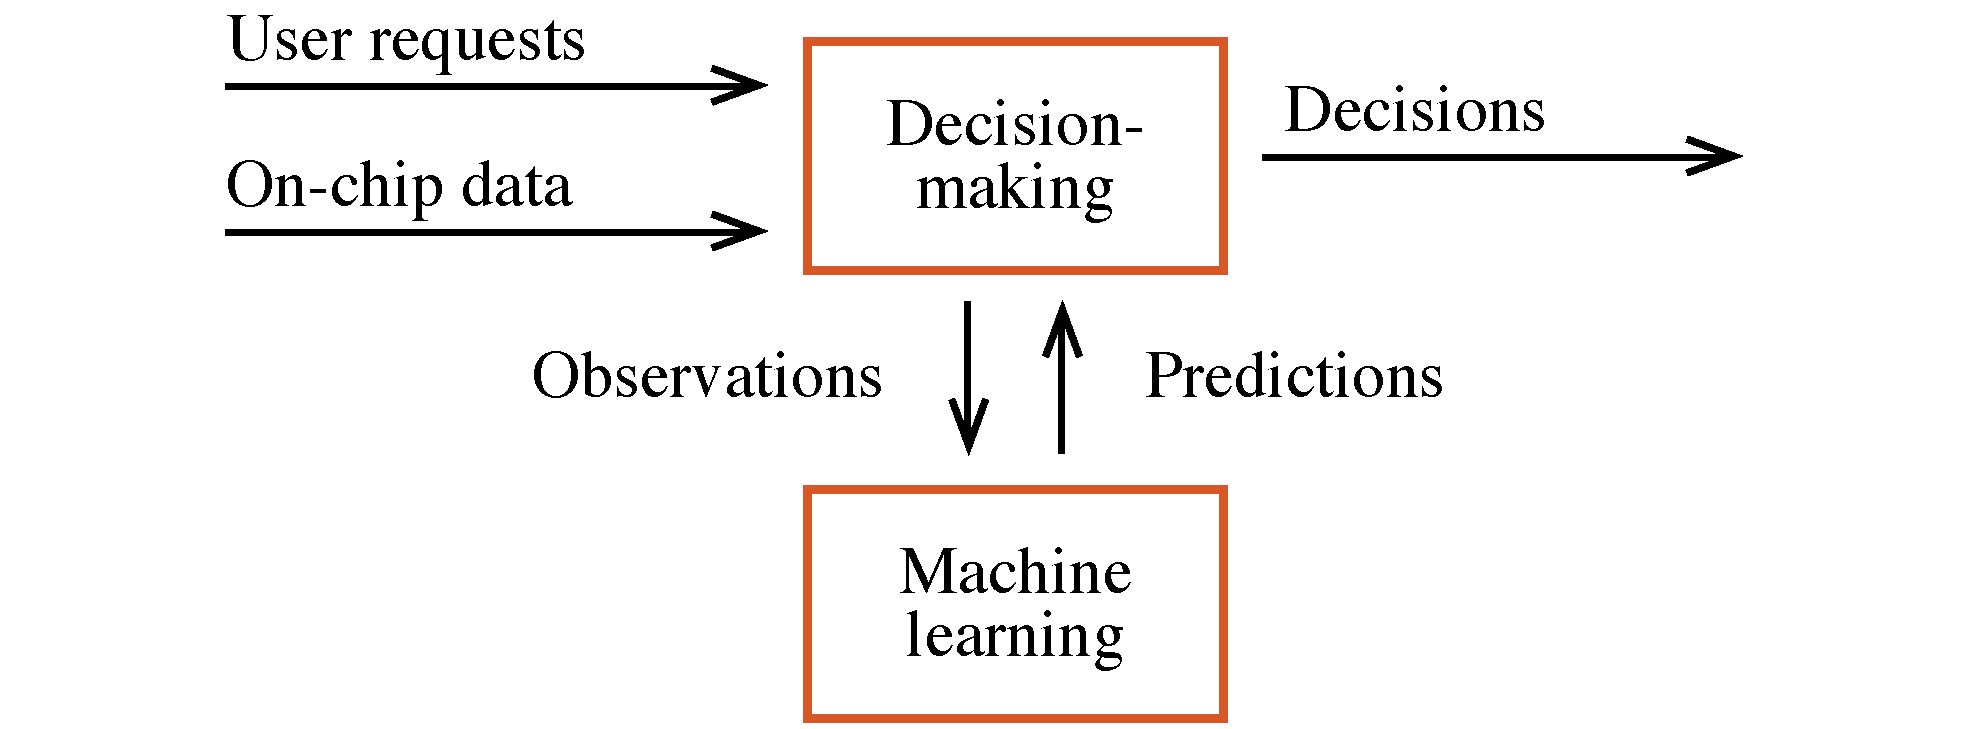
\includegraphics[width=1.0\columnwidth]{include/assets/figures/governor.pdf}

  \caption{A proactive governor of an electronic system. \emph{Observations}
  refers to the data used for learning. \emph{Predictions} refers to the data
  that the management strategy needs to know in advance in order to make
  proactive decisions.}

  \flab{governor}
\end{figure}

So far we have obtained two corresponding streams: arrival and workload. The two
streams merge into a new stream representing a sequence of concrete incoming
jobs or user requests, and this new stream needs to be processed, which is the
topic of this subsections. Here, \emph{processing} refers to progressively
building a schedule,\footnote{In this paper, mapping is assumed to be a part of
scheduling.} constructing a power profile, and computing the corresponding
temperature profile. In \fref{methodology}, this functionality resides in the
box labeled ``Streamer.''

As motivated in \sref{motivation}, a prominent use case of our methodology is
the development of management strategies. Therefore, the management core of the
system at hand is devised by the user, which is further detailed in
\sref{usage}. Hence, a scheduling policy is given, and it decides on a schedule.
Namely, each arrived job contains information about the computational resources
it needs, and the policy specifies when the job gets access to these resources.
Then we add accordingly the recorded (and potentially transformed) power pattern
of the job to the power profile of the system. A helpful analogy here might be
paving a road with rectangular bricks of different sizes. As the time goes by,
we feed the power profile to a temperature simulator and obtain a temperature
profile.

The power and temperature profiles are the final output of our methodology. The
key observation to be made is that no prohibitively expensive performance or
power simulations are involved in the data-synthesis stage. The time consumed by
the procedure delineated above is practically negligible.

At this point, we would like to draw attention to the following. It should be
clear that, by recording power directly, we make a trade-off, and making this
trade-off is necessary. Many details pertaining to programs' executions have
been discarded in order to gain speed. What has been baked into recordings
cannot be to altered at the data-synthesis stage in general. Consider, for
instance, a recording of a program that had two cores at its disposal. This
pattern cannot be used to replay the execution as if there was only one core.
Similarly, the recording cannot tell what would happen if the program could
leverage one additional core. Another limitation concerns resource sharing,
which is twofold. First, workload patterns obtained in isolation cannot used to
fabricate the interleaving of two programs (time sharing). Second, even if two
programs run on two different cores, they still can affect each other by
competing for such resources as shared L3 caches. Currently, the above concerns
can be addresses in our methodology only partially.
